\documentclass[aspectratio=169,10pt]{beamer}
\usepackage[spanish]{babel}
\usepackage[utf8]{inputenc}
\usepackage[T1]{fontenc}
\usepackage{booktabs,array,tikz,xcolor}
\usetikzlibrary{positioning,arrows.meta,shapes.geometric}

\definecolor{azul}{HTML}{1F3A5F}
\definecolor{acento}{HTML}{E07A2F}
\definecolor{gris}{HTML}{5B6670}
\definecolor{verde}{HTML}{2E7D4F}
\definecolor{rojo}{HTML}{B83232}

\usetheme{default}
\usefonttheme{professionalfonts}
\setbeamercolor{frametitle}{fg=azul}
\setbeamercolor{title}{fg=azul}
\setbeamercolor{itemize item}{fg=acento}
\setbeamercolor{itemize subitem}{fg=acento}
\setbeamerfont{frametitle}{series=\bfseries,size=\Large}
\setbeamertemplate{navigation symbols}{}
\setbeamertemplate{footline}{\hfill\color{gris}\footnotesize\the\numexpr\insertframenumber-1\relax\,/\,10\hspace{1em}\vspace{0.4em}}
\setbeamertemplate{itemize items}[circle]
\setbeamersize{text margin left=1.2em,text margin right=1.2em}

\newcommand{\dato}[2]{{\Large\bfseries\color{acento}#1}\\[-0.2em]{\footnotesize\color{gris}#2}}

\title{Optimización logística: pronóstico y plan de entrega}
\subtitle{Desafío técnico Data Scientist Lead}
\date{Octubre 2026}

\begin{document}

\begin{frame}[plain]
\titlepage
\end{frame}

% 1
\begin{frame}{1. El pronóstico actual falla por sesgo, no por ruido}
\small
\begin{center}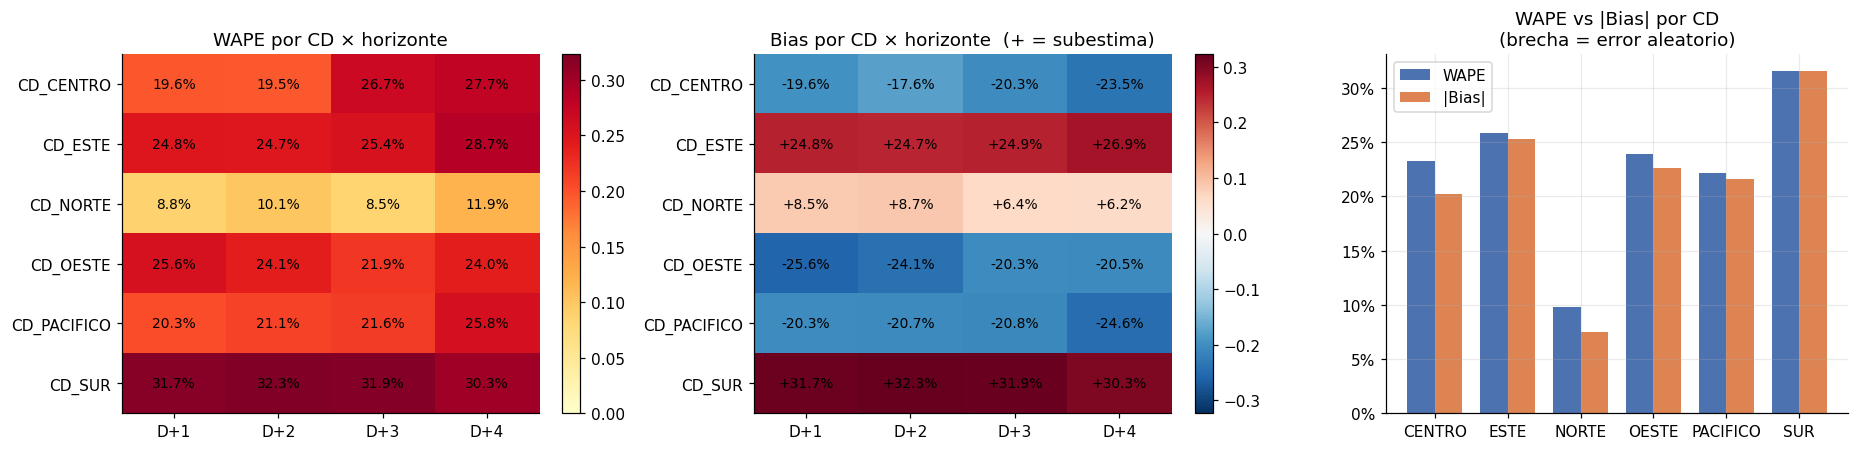
\includegraphics[width=0.8\textwidth]{img/diagnostico.png}\end{center}
\begin{columns}[T]
\column{0.5\textwidth}
\textbf{Subestiman} (riesgo de flete de emergencia)
\begin{itemize}
\item CD\_SUR \textcolor{rojo}{+31,6\%}, CD\_ESTE \textcolor{rojo}{+25,3\%}, CD\_NORTE +7,5\%
\end{itemize}
\column{0.5\textwidth}
\textbf{Sobreestiman} (flota ociosa)
\begin{itemize}
\item CD\_OESTE \textcolor{azul}{$-22,7\%$}, CD\_PACIFICO $-21,6\%$, CD\_CENTRO $-20,2\%$
\end{itemize}
\end{columns}
\vspace{0.3em}
\begin{itemize}
\item El signo es el mismo en los 4 horizontes y en los 6 CDs.
\item En CD\_SUR el WAPE es igual al Bias: el pronóstico quedó bajo la demanda todos los días.
\item Solo CD\_NORTE está bien calibrado (WAPE 9,8\%).
\end{itemize}
\end{frame}

% 2
\begin{frame}{2. La precisión baja con el horizonte, pero poco}
\begin{columns}[T]
\column{0.5\textwidth}
\begin{center}
\begin{tabular}{lrr}
\toprule
Horizonte & WAPE & Bias \\
\midrule
D+1 & 19,8\% & +6,9\% \\
D+2 & 20,3\% & +7,6\% \\
D+3 & 20,9\% & +6,4\% \\
D+4 & 22,5\% & +5,2\% \\
\midrule
Global & 20,8\% & +6,6\% \\
\bottomrule
\end{tabular}
\end{center}
\vspace{0.5em}
\begin{itemize}
\item De D+1 a D+4 el error sube 2,8 puntos (+14\% relativo).
\item Casi plano hasta D+3, y salta en D+4.
\end{itemize}
\column{0.5\textwidth}
\begin{center}
\begin{tabular}{lrrr}
\toprule
CD & WAPE & Bias & \% días sub. \\
\midrule
SUR & 31,6\% & +31,6\% & 100\% \\
ESTE & 25,9\% & +25,3\% & 95\% \\
NORTE & 9,8\% & +7,5\% & 80\% \\
CENTRO & 23,3\% & $-20,2\%$ & 11\% \\
PACIFICO & 22,2\% & $-21,6\%$ & 5\% \\
OESTE & 23,9\% & $-22,7\%$ & 7\% \\
\bottomrule
\end{tabular}
\end{center}
\end{columns}
\vspace{0.8em}
\begin{block}{Lo que importa}
Casi todo el error es sesgo de nivel por CD. Antes de pensar en un modelo complejo, hay que recalibrar.
\end{block}
\end{frame}

% 3
\begin{frame}{3. El plan de entrega se queda corto y se atrasa}
\begin{columns}[T]
\column{0.33\textwidth}
\dato{+10,6\%}{volumen real sobre el plan\\(78,9k vs 70,5k unidades)}
\column{0.33\textwidth}
\dato{17,5\%}{de las compras fuera de plan\\(21\% del volumen)}
\column{0.33\textwidth}
\dato{+2,5 días}{desfase medio\\77\% se compra después}
\end{columns}
\vspace{0.8em}
\begin{columns}[T]
\column{0.55\textwidth}
\begin{itemize}
\item En 71\% de las compras el cliente pidió más de lo planificado.
\item El sesgo de volumen se ve en todos los CDs y canales (8\% a 14\%).
\item Los desvíos son más grandes: el volumen fuera de plan tiene un sesgo de +16,9\%.
\end{itemize}
\column{0.45\textwidth}
\begin{center}
\begin{tabular}{lr}
\toprule
CD & \% fuera de plan \\
\midrule
NORTE & 24,4\% \\
PACIFICO & 21,3\% \\
ESTE & 19,5\% \\
SUR & 18,9\% \\
CENTRO & 11,1\% \\
OESTE & 10,2\% \\
\bottomrule
\end{tabular}
\end{center}
\end{columns}
\vspace{0.3em}
{\footnotesize\color{gris} Por día planificado: lunes 22\%, martes 16\%, miércoles 23\%, jueves 14\%, viernes 16\%. La diferencia entre días no es concluyente con esta muestra (p = 0,22).}
\end{frame}

% 4
\begin{frame}{4. Pocos clientes se desvían y todos corren hacia el martes}
\small
\begin{center}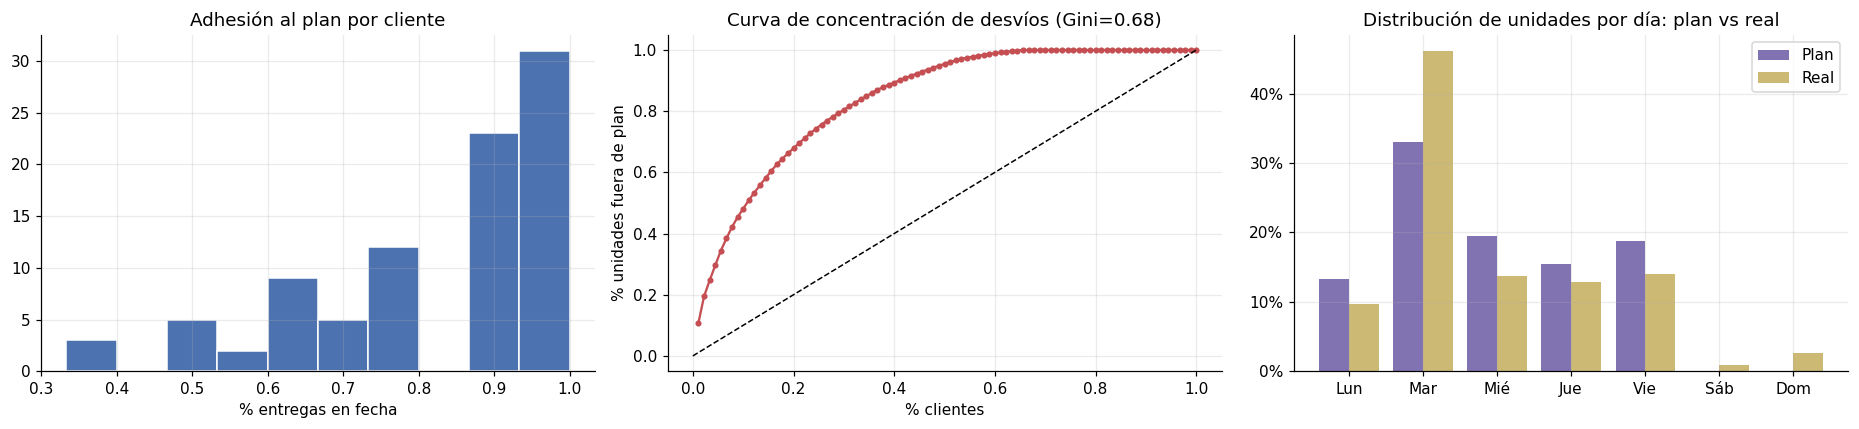
\includegraphics[width=0.68\textwidth]{img/plan.png}\end{center}
\vspace{-0.2em}
\begin{columns}[T]
\column{0.45\textwidth}
\textbf{Qué vemos}
\begin{itemize}
\item Adhesión media de 82\%. 20 de 90 clientes bajo 70\%.
\item El 10\% de los clientes explica 48\% de las unidades fuera de plan.
\item El martes pasa de 33\% a 46\% del volumen.
\end{itemize}
\column{0.55\textwidth}
\textbf{Qué proponemos: fecha dinámica con incentivo}
\begin{itemize}
\item Al cotizar, recomendar la fecha de menor utilización dentro de la ventana del cliente (±1 a 3 días).
\item Incentivo pequeño en días valle y tope blando de 90\% por CD-día.
\item Partir por los clientes más inestables y medir con A/B.
\end{itemize}
\end{columns}
\vspace{0.3em}
\textbf{Ojo:} en simulación, mover 10\% de la carga excedente baja los CD-días sobre 90\% de 18\% a 4\%, pero el peak-to-average solo pasa de 1,27 a 1,23 y el martes casi no cambia. Ayuda más a evitar pasarse de capacidad que a aplanar.

\textbf{KPIs:} \% de CD-días sobre 90\%, peak-to-average, share del martes, tasa de aceptación.
\end{frame}

% 5
\begin{frame}{5. Modelo de corrección: simple y sin fuga de datos}
\begin{columns}[T]
\column{0.5\textwidth}
\textbf{Idea}
\begin{itemize}
\item Se predice $\log(\text{real}/\text{pronóstico base})$ y se corrige: $\text{fc}_{corr}=\text{fc}_{base}\cdot e^{\hat y}$.
\item Se limita la corrección a un ratio entre 0,5 y 2,0.
\item Solo se usan datos conocidos al día de emisión (hay un test automático de no fuga).
\end{itemize}
\textbf{Modelos comparados}
\begin{itemize}
\item Recalibración por CD (razón histórica)
\item Ridge (propuesto)
\item HistGradientBoosting (challenger)
\end{itemize}
\column{0.5\textwidth}
\textbf{Variables}
\begin{itemize}
\item Base: pronóstico, horizonte, CD
\item Calendario: día de semana, martes, fin de semana, pico de hace 7 días, pronóstico sobre capacidad
\item Rolling: media y desviación móvil 7 y 14 días
\item Error reciente del modelo base por CD y horizonte
\end{itemize}
\textbf{Validación}
\begin{itemize}
\item Origen rodante, 5 folds semanales
\item 708 pronósticos fuera de muestra (29 ene a 28 feb)
\end{itemize}
\end{columns}
\end{frame}

% 6
\begin{frame}{6. El WAPE baja de 20,7\% a 7,2\%}
\small
\begin{center}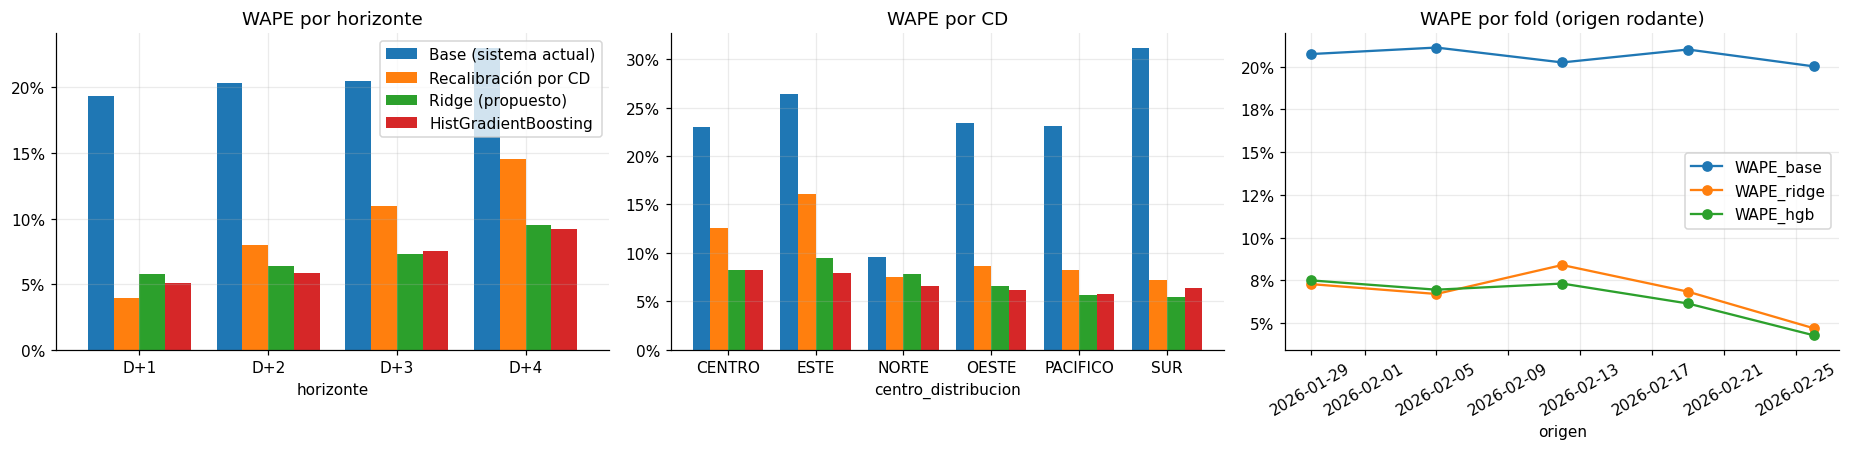
\includegraphics[width=0.68\textwidth]{img/modelo.png}\end{center}
\vspace{-0.2em}
\begin{columns}[T]
\column{0.5\textwidth}
\begin{center}
\small
\begin{tabular}{lrr}
\toprule
Modelo & WAPE & Bias \\
\midrule
Base actual & 20,7\% & +6,7\% \\
Recalibración por CD & 9,2\% & +0,0\% \\
Ridge (propuesto) & 7,2\% & +1,0\% \\
HistGradientBoosting & 6,9\% & +1,2\% \\
\bottomrule
\end{tabular}
\end{center}
\column{0.5\textwidth}
\begin{itemize}
\item Mejora de 13,5 puntos, IC95\% [12,3 ; 14,7].
\item Gana en los 5 folds, 4 horizontes y 6 CDs.
\item 85\% de la mejora viene de quitar el sesgo por CD.
\end{itemize}
\end{columns}
\vspace{0.3em}
\begin{alertblock}{Ojo}
En D+1 la recalibración simple (4,0\%) le gana al Ridge (5,8\%). Las rolling features no aportan mejora medible. Los datos parecen sintéticos, con un sesgo estable por CD, y son solo 60 días: en producción esperaría una mejora menor.
\end{alertblock}
\end{frame}

% 7
\begin{frame}{7. Arquitectura en AWS}
\centering
\begin{tikzpicture}[scale=0.85,transform shape,
  node distance=0.55cm and 0.7cm,
  box/.style={draw=azul,fill=azul!8,rounded corners=2pt,align=center,font=\scriptsize,minimum height=0.9cm,minimum width=2.3cm},
  store/.style={box,fill=acento!15,draw=acento},
  gate/.style={box,fill=verde!15,draw=verde},
  lab/.style={font=\scriptsize\bfseries\color{gris}},
  arr/.style={-{Stealth[length=4pt]},color=gris}]
\node[box] (src) at (0,0) {Plataforma B2B\\pedidos, plan,\\pronóstico, capacidad};
\node[box] (s3) at (2.9,0) {Kinesis Firehose\\$\rightarrow$ S3 raw};
\node[box] (glue) at (5.8,0) {Glue / Athena\\features rolling};
\node[gate] (gate) at (8.7,0) {Lambda\\Gate de 45 días};
\node[box] (sm) at (11.6,0) {SageMaker Training\\+ Model Registry};
\node[box] (eb) at (5.8,1.6) {EventBridge\\+ Step Functions};
\node[box] (app) at (0,-2.3) {App backend / web};
\node[box] (api) at (2.9,-2.3) {API Gateway\\+ Lambda\\recomendar fecha};
\node[store] (ddb) at (8.7,-2.3) {DynamoDB\\estado Gate, modelo,\\carga comprometida};
\node[store] (s3c) at (11.6,-2.3) {S3 curated\\modelos y métricas};
\node[box] (cw) at (14.5,-2.3) {CloudWatch + SNS\\alarmas de Bias y Gate};
\draw[arr] (src)--(s3); \draw[arr] (s3)--(glue); \draw[arr] (glue)--(gate); \draw[arr] (gate)--(sm);
\draw[arr] (eb)--(glue);
\draw[arr] (gate)--(ddb);
\draw[arr] (sm)--(s3c);
\draw[arr] (app)--(api);
\draw[arr] (api)--(ddb);
\draw[arr] (s3c.south)--++(0,-0.5)-|(api.south);
\draw[arr] (s3c)--(cw);
\node[lab,above=0.05cm of eb] {Batch diario y semanal};
\end{tikzpicture}
\vspace{0.3em}
\begin{itemize}\scriptsize
\item \textbf{Batch:} cada día se calculan features y el Gate; cada semana se reentrena y solo se promueve el modelo si le gana al base en backtest.
\item \textbf{Inferencia:} el endpoint siempre responde. Si el CD está en fallback, devuelve el pronóstico base.
\item \textbf{Persistencia:} cada recomendación guarda versión de modelo, estado del Gate y fecha de corte.
\end{itemize}
\end{frame}

% 8
\begin{frame}{8. Gate de 45 días: qué pasa si se mueve el umbral}
\small
\begin{center}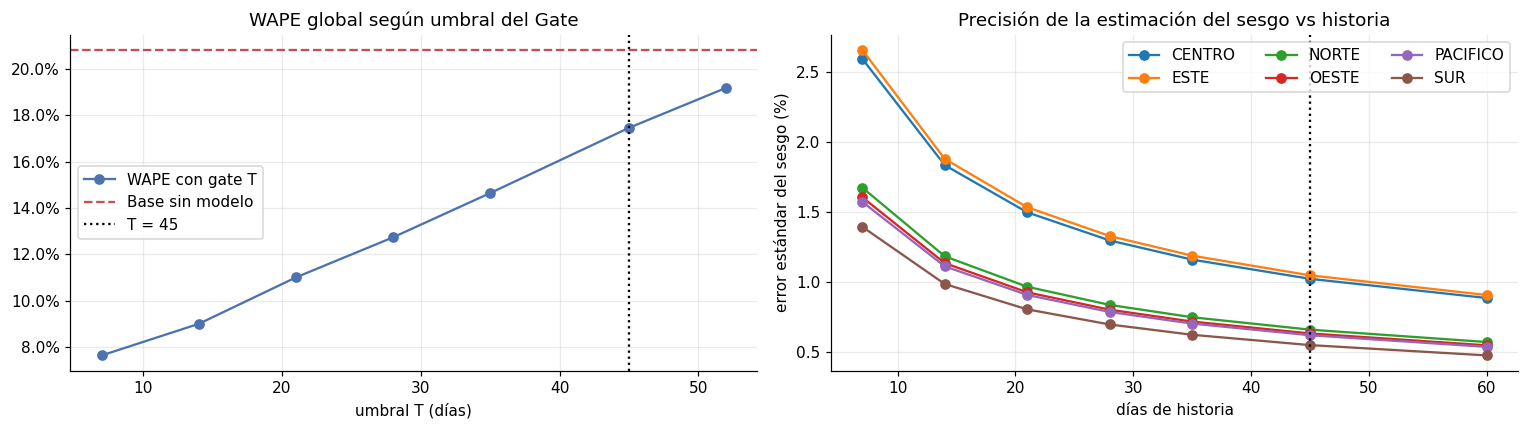
\includegraphics[width=0.7\textwidth]{img/gate.png}\end{center}
\vspace{-0.2em}
\begin{columns}[T]
\column{0.5\textwidth}
\textbf{Regla}
\begin{itemize}
\item Historia continua $\ge$ 45 días: entrena y corrige.
\item Menos de 45, hueco reciente o sin datos: pronóstico base, con el motivo registrado. Nunca lanza excepción.
\item Se evalúa por CD y todos los días.
\end{itemize}
\column{0.5\textwidth}
\textbf{Qué dicen los datos}
\begin{itemize}
\item Con T = 45 el WAPE es 17,5\%. Con T = 14 sería 9,0\%.
\item El sesgo se detecta con 1 a 3 días, así que 45 es conservador.
\item Riesgo de bajarlo: con 14 días hay 2 datos por día de semana y se puede sobre-corregir algo transitorio.
\end{itemize}
\end{columns}
\vspace{0.2em}
\textbf{Recomendación:} mantener 45 para activar todo y agregar un modo intermedio entre 14 y 44 días, solo con recalibración por CD y la mitad del ajuste.
\end{frame}

% 9
\begin{frame}{9. Impacto en el negocio}
\begin{columns}[T]
\column{0.55\textwidth}
\begin{center}
\small
\begin{tabular}{lrrr}
\toprule
Colchón de flota & 0\% & 5\% & 10\% \\
\midrule
Flete emergencia & $-70\%$ & $-81\%$ & $-87\%$ \\
Fill rate (pp) & +9,7 & +9,2 & +8,2 \\
Costo total & $-8\%$ & $-6\%$ & $-3\%$ \\
Capacidad ociosa & $-32\%$ & +8\% & +44\% \\
\bottomrule
\end{tabular}
\end{center}
{\footnotesize\color{gris} Base contra corregido, fuera de muestra. Supuesto: flete de emergencia cuesta 1,8 veces la flota planificada.}
\column{0.45\textwidth}
\begin{itemize}
\item Con colchón de 5\%, el fill rate pasa de 88,6\% a 97,8\%.
\item El ahorro se mantiene con tarifas de 1,5 a 3 veces y crece con el sobrecosto.
\item CD\_SUR y CD\_ESTE concentran la mejora.
\end{itemize}
\end{columns}
\vspace{0.5em}
\begin{alertblock}{Ojo}
No es gratis. En CD\_CENTRO los fletes de emergencia suben, porque el sesgo de sobreestimación hacía de colchón. El modelo corregido necesita menos colchón que el base: con 10\% sobra flota.
\end{alertblock}
\end{frame}

% 10
\begin{frame}{10. KPIs, límites y próximos pasos}
\begin{columns}[T]
\column{0.6\textwidth}
\textbf{KPIs}
\begin{center}
\footnotesize
\begin{tabular}{p{2.0cm}p{5.2cm}}
\toprule
Precisión & WAPE y Bias por CD y horizonte (7 y 28 días). Meta: Bias entre $-5\%$ y +5\% \\
Costo & \% de unidades en flete de emergencia, costo por unidad \\
Flota & \% de capacidad contratada ociosa \\
Servicio & Fill rate / OTIF por CD \\
Aplanamiento & Peak-to-average, CD-días sobre 90\% de capacidad, share del martes \\
Plan & Adhesión y Bias de volumen del plan \\
Gate & \% de CD-días en fallback \\
\bottomrule
\end{tabular}
\end{center}
\column{0.4\textwidth}
\textbf{Límites}
\begin{itemize}
\item Solo 60 días: sin estacionalidad ni festivos.
\item Datos que parecen sintéticos, con sesgo estable por CD.
\item Costos con supuestos, no con tarifas reales.
\item El plan cubre 90 clientes (cerca de 15\% del volumen).
\end{itemize}
\textbf{Próximos pasos}
\begin{itemize}
\item Validar con más historia y tarifas reales.
\item Modelo o mezcla por horizonte.
\item Piloto A/B de fecha dinámica en CD\_NORTE.
\end{itemize}
\end{columns}
\end{frame}

\end{document}
